% Compile using: TEXINPUTS=minted/source: xelatex -shell-escape slides.tex
\documentclass[12pt,compress,english,utf8,t]{beamer}

\usepackage{etex}

\usepackage[english]{babel}

\usepackage{tikz}
\usepackage{booktabs}
\usepackage{ragged2e}
\usepackage[normalem]{ulem}

\makeatletter
\ifbeamer@draftmode
\usepackage{verbatim}
\newcommand{\inputminted}[2]{\verbatiminput{#2}}
\else
\usepackage{minted}
\setminted{linenos}
\fi
\makeatother

\usetikzlibrary{calc,shapes.callouts,shapes.arrows}
\definecolor{darkred}{RGB}{220,0,0}
\newcommand{\hcancel}[5]{%
    \tikz[baseline=(tocancel.base)]{
        \node[inner sep=0pt,outer sep=0pt] (tocancel) {#1};
        \draw[darkred, line width=1mm] ($(tocancel.south west)+(#2,#3)$) -- ($(tocancel.north east)+(#4,#5)$);
    }%
}%

\usepackage[protrusion=true,expansion=false]{microtype}

\usepackage{fontspec}
\newfontfamily\DejaSans{DejaVu Sans}

\title[Pugs, an experimental Perl 6 platform: a retrospective]{
  \raisebox{-0.3mm}{\DejaSans ☺}
  A retrospective on Pugs
  \raisebox{-0.3mm}{\DejaSans ☺}
}
\author[Augsburg.pm (April 13th, 2015)]{\texorpdfstring{
  \vspace{-0.5em} \\
  
\includegraphics[scale=0.3]{images/lambdacamel-small} \\[0.5em]
  Ingo Blechschmidt \\
  \scriptsize \texttt{<iblech@speicherleck.de>}
}{Ingo Blechschmidt}}
\date{April 13th, 2015}

\usetheme{Warsaw}
\usecolortheme{seahorse}
\definecolor{mypurple}{RGB}{60,0,255}
\setbeamercolor{structure}{fg=mypurple}
\usefonttheme{serif}
\usepackage{fontspec}
\defaultfontfeatures{Mapping=tex-text}
\setmainfont{Linux Libertine O}
\useinnertheme{rectangles}
\setbeamercovered{invisible}

\setbeamertemplate{title page}[default][colsep=-1bp,rounded=false,shadow=false]
\setbeamertemplate{frametitle}[default][colsep=-2bp,rounded=false,shadow=false,center]

\setbeamertemplate{navigation symbols}{}
\setbeamertemplate{headline}{}

\newcommand*\oldmacro{}%
\let\oldmacro\insertshorttitle%
\renewcommand*\insertshorttitle{%
  \oldmacro\hfill\insertframenumber\,/\,\inserttotalframenumber\hfill}

\newcommand{\hil}[1]{{\usebeamercolor[fg]{item}{\textbf{#1}}}}

\newcommand{\atpos}[1]{%
  \begin{tikzpicture}[remember picture, overlay]%
    \node[anchor=south east] at (current page.south east) {#1};
  \end{tikzpicture}%
}

\newcommand{\centeredpar}[2]{%
  \begin{center}
    \colorbox{white}{\parbox{#1\textwidth}{%
      #2%
    }}%
  \end{center}%
}

\newcommand{\sourcedquote}[4]{%
  ``#1''\par%
  {\raggedleft -- #2, #3, \href{#4}{\underline{link}}\par}%
}

% Gonzalo Medina, http://tex.stackexchange.com/a/228198
\makeatletter
\def\Mdescription#1{%
  \advance\beamer@descdefault by \labelsep%
  \list
  {}
  {\labelwidth\beamer@descdefault%
  \leftmargin\beamer@descdefault%
  \let\makelabel\beamer@descriptionitem
  \settowidth\labelwidth{\beamer@descriptionitem{#1}}%
  \setlength\leftmargin{\labelwidth}% 
  \addtolength\leftmargin{\labelsep}%
  }%
  \beamer@cramped%
  \raggedright
  \beamer@firstlineitemizeunskip%
}
\def\endMdescription{\ifhmode\unskip\fi\endlist}
\long\def\beamer@descriptionitem#1{%
  \def\insertdescriptionitem{#1}%
  {\usebeamertemplate**{description item}}\hfil}
\makeatother

\setbeameroption{show notes}
\setbeamertemplate{note page}[plain]

\begin{document}

\frame{\titlepage}

\frame[plain]{
  \centeredpar{0.9}{
    \justifying\scriptsize
    \textbf{Abstract.}
    ``Hi. Today I have started working on specifying and implementing
    Featherweight Perl 6 (FP6), a side-effect-free subset of Perl~6.''
    Audrey Tang used these words to unveil the Pugs project in February of 2005.
    Initially conceived as an implementation of a small subset of Perl~6 in
    Haskell, the project quickly grew to contain a full-fledged compiler and
    interpreter for Perl~6 and attracted a large and diverse community.

    \medskip
    The talk will give a subjective survey of the history of Pugs. We will pay
    particular attention to the special manner with which Audrey led the project and
    what the philosophy ``-O\emph{fun}'' meant to the developers. We'll also discuss
    which parts of Pugs were absorbed into other implementations of Perl~6 and
    which influence Pugs had on the Perl and Haskell communities.
    \medskip

    \textbf{About me.} I contributed to Pugs as a school student in
    2005, at first by porting modules and writing tests, then gradually also by
    writing Haskell code and later by implementing a JavaScript backend. Audrey
    and the unique spirit in the Pugs community had a strong and lasting
    influence on me (exposing me to Haskell, category theory, and
    a beautiful way of tending communities); I look back on very exciting and
    fun days.
    \medskip

    \textbf{Warning.} The account is mostly from memory and not properly
    researched. Try not to trust it! Also note that the timeline covers only
    the year 2005 and that \emph{the code excerpts are
    edited for legibility}, i.\,e.\@ shortened at a few places and not
    reproduced verbatim. Pull requests are very much welcome; in fact, in good
    old Pugs spirit you will get full write access to the repository so you
    can merge them yourself.
    \medskip

    \centering
    \url{https://github.com/iblech/talk-pugs-retrospective}
    \par
  }
}

\setcounter{tocdepth}{2}
\frame{\tableofcontents}

\section{A glimpse of Perl 6}

\begin{frame}[fragile]\frametitle{A glimpse of Perl 6}
  \only<1>{\inputminted{perl}{code-snippets/a-glimpse-of-perl6-1.pl}}
  \only<2>{\inputminted{perl}{code-snippets/a-glimpse-of-perl6-2.pl}}
  \pause
  \pause

  \justifying
  closures \textbullet{}
  anonymous types \textbullet{}
  roles and traits \textbullet{}
  named arguments \textbullet{}
  expressive subroutine and method signatures \textbullet{}
  a strong meta object system \textbullet{}
  macros \textbullet{}
  state variables \textbullet{}
  cleaned up regular expressions \textbullet{}
  named regexes for easy reuse \textbullet{}
  grammars for parsing \textbullet{}
  lazy lists \textbullet{}
  junctions of values \textbullet{}
  optional type annotations (gradual typing) \textbullet{}
  powerful run-time multi dispatch \textbullet{}
  lexical imports
  \par
\end{frame}

\begin{frame}
  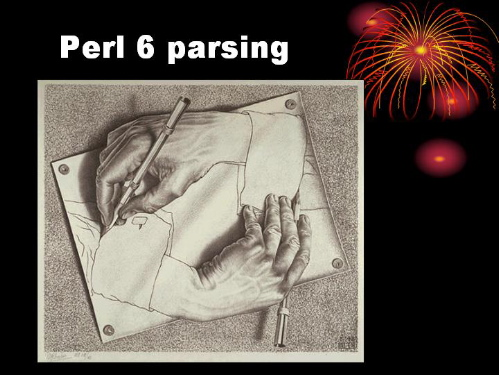
\includegraphics[width=0.45\textwidth]{images/perl-6-parsing.jpeg}

  \hfill
\includegraphics[width=0.45\textwidth]{images/implementing-perl-6.jpeg}
\end{frame}

\section{Timeline of Pugs development}

\subsection{The beginning}

\logo{
\includegraphics[scale=0.13]{images/audreyt2.jpeg}}
\begin{frame}\frametitle{The beginning}
  \vspace*{-1em}
  \centeredpar{0.9}{
    \hil{``Hi. Today I have started working on specifying and implementing
    Featherweight Perl 6 (FP6), a side-effect-free subset of Perl~6.''}

    \raggedleft -- Audrey Tang, February 2nd, 2005,
    \href{http://www.nntp.perl.org/group/perl.perl6.language/2005/02/msg19013.html}{\underline{link}}
  }

  \begin{Mdescription}{2001}
    \item[2001] Apocalypse 1, first Perl 6 design document
    \item[2004] Many Apocalypse and Synopse documents
    \item[2005] Active discussion on perl6-language@perl.org
    \item[2005] Pugs, providing the first usable implementation
    \item[]
    \item[2005] Facebook
    \item[2005] YouTube
    \item[2008] GitHub
  \end{Mdescription}
\end{frame}
\logo{}

\begin{frame}\frametitle{Haskell?}
  \begin{center}
    \vbox{
\includegraphics[width=0.35\textwidth]{images/haskell-meme-2.jpeg}
\includegraphics[width=0.35\textwidth]{images/haskell-meme-4.jpeg}\\
    
\includegraphics[width=0.35\textwidth]{images/haskell-meme-5.jpeg}
\includegraphics[width=0.35\textwidth]{images/haskell-meme-6.jpeg}}
  \end{center}
\end{frame}

% http://wayback.archive.org/web/20050209100505/http://haskell.org/hawiki/Perl6UsersGolfingSystem
\begin{frame}[fragile]\frametitle{Screenshot}\scriptsize
  \vspace{-2.0em}
  \begin{verbatim}.=====. __  __  ____   ___    _________________________________________
||   || ||  || ||  || ||__'   Pugs 6: Based on the Perl 6 Synopses
||====' ||__|| ||__||  __||   Copyright (c) 2005 Autrijus Tang
||      `===='  ___|| `==='   World Wide Web: http://autrijus.org/pugs
||             `===='         Report bugs to: autrijus@autrijus.org
==           Version: 6.0.0   =========================================

Welcome to Pugs -- Perl6 User's Golfing System
Type :h for help

pugs> :h
Commands available from the prompt:
:h              = show this help message
:q              = quit
. <exp>         = show the syntax tree of an expression
? <exp>         = evaluate an expression

pugs> . ('1' & "2") * (3.0 | "4abcd")
Op2 "*" (Op2 "&" (Val (VStr "1")) (Val (VStr "2"))) (Op2 "|" (Val (VNum 3.0)) (Val (VStr "4abcd")))

pugs> ('1' & "2") * (3.0 | "4abcd")
((3.0 | 4.0) & (6.0 | 8.0))

pugs> :q
Leaving pugs.\end{verbatim}
\end{frame}

\note{
  \begin{itemize}
    \justifying
    \item \sourcedquote{As I'm finding my way through TaPL and ATTaPL today, it occurs to me that
    I should implement a real language as an exercise; that real language turns
    out to be Perl~6. So it begins \ldots}{Audrey Tang}{February 1st,
    2005}{http://wayback.archive.org/web/20050206202119/http://use.perl.org/~autrijus/journal/}
    \item TaPL refers to \emph{Types and Programming Languages}, a
    computer-science book on implementing programming languages.
    \item Audrey quickly dropped her initial plan to focus on a
    side-effect-free subset (on day~3, to be precise).
    \item There was an implementation before Pugs, a tiny
    project sitting in the Parrot source tree.
    \item Audrey's first post contained a language semantics question. This
    would be the beginning of continuing refinements of the specification, made
    possible by the existence of a useful Perl~6 platform which allowed people
    to play with Perl~6.
  \end{itemize}
}

\note{
  \begin{itemize}
    \justifying
    \item \sourcedquote{This last year, we were starting to lose our sense of
    fun in the Perl community. Though we tried to be careful about not making
    promises, everyone knew in their hearts that five years is an awfully long
    time to wait for anything. People were getting tired and discouraged and a
    little bit dreary.

    Then [Audrey Tang] showed up.}{Larry Wall}{August
    2005 (OSCON)}{http://www.perl.com/pub/2005/09/22/onion.html}
  \end{itemize}

  \begin{center}
    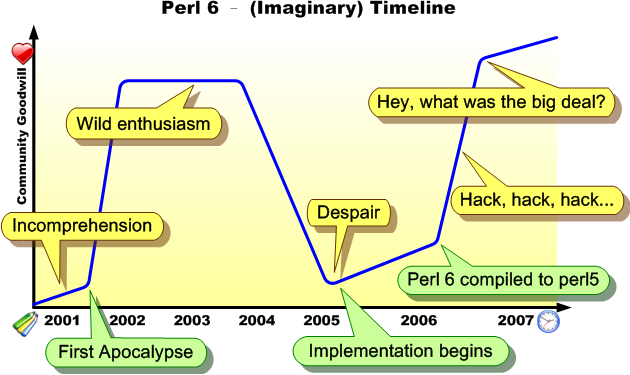
\includegraphics[scale=0.35]{images/timeline}
  \end{center}
}

\note{
  \#haskell on 2009-04-17, discussion about (AT)TaPL, \href{http://ircbrowse.net/browse/haskell?id=7390873}{\underline{link}}:
  \begin{tabbing}
    \hil{$\langle$edwardk$\rangle$} \= \kill
    \hil{$\langle$edwardk$\rangle$} \> shapr recommended it to audreyt and
    audrey went off and \\
    \> wrote pugs to work through the processes in the book
  \end{tabbing}

  So, thank you shapr!
}


\subsection{The early days}

\begin{frame}[label=the-early-days]\frametitle{The early days}
  \begin{Mdescription}{Day 00}
    \item[Day 4] ``Parsec; 90\,\% of operators implemented!''
    \hfill\hyperlink{parsec}{\beamerbutton{see code}}
    \item[Day 8] ``Pugs 6.0.2; Turing Completeness''
    \hfill\hyperlink{turing-completeness}{\beamerbutton{see code}}
    \item[Day 12] ``Refactoring''
    \hfill\hyperlink{refactoring}{\beamerbutton{see code}}
    \item[Day 13] ``Continuations''
    \hfill\hyperlink{continuations}{\beamerbutton{see code}}
    \item[Day 14] ``All tests successful''
    \hfill\hyperlink{all-tests-successful}{\beamerbutton{see code}}
    \item[Day 20] ``6.0.8''
    \hfill\hyperlink{608}{\beamerbutton{see code}}
    \item[Day 23] ``Test.pm flies!''
    \hfill\hyperlink{testpm}{\beamerbutton{see code}}
  \end{Mdescription}

  \hyperlink{further-highlights}{\beamerbutton{skip details}}
\end{frame}

\note{
  \justifying
  As can be seen by the journal headlines, Pugs was extremely fast-moving. In
  the early days, a Pugs build of a day ago was considered to be vastly
  outdated. This had two reasons:
  \begin{itemize}
    \justifying
    \item Firstly, Audrey was an astoundingly productive hacker, rapidly
    implementing major features and attracting a large community of fellow
    \emph{lambdacamels} (totaling more than~200 contributors).
    \item Secondly, Haskell's unique features rendered it a very fine language
    for implementing other languages. It allowed both for quick prototyping and easy
    refactoring.
  \end{itemize}
  See the \href{http://irclog.perlgeek.de/perl6/2005-03-02}{logs of
  \#perl6 for 2005-03-02 (\underline{link})} for an interesting chat between Audrey and
  chromatic, among other things about Pugs's beginnings and Haskell's
  strengths. Highly recomended reading.
  \par
}

\note{
  \begin{center}
    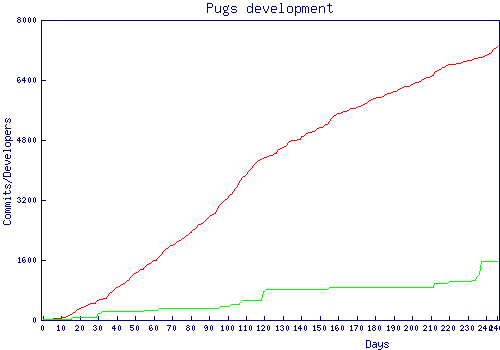
\includegraphics[scale=0.45]{images/pugs-svngraph-6.2.10.png}
  \end{center}

  \begin{itemize}
    \justifying
    \item This graph was made at the release of Pugs~6.2.10. The red curve
    shows the absolute number of commits, the green one shows the number of
    committers -- multiplied by~10.
    \item This graph is by far not the nicest graph in the history of graphs.
  \end{itemize}
}

\logo{\hyperlink{the-early-days}{\beamerbutton{Continue slides \ldots}}}

\begin{frame}[label=parsec]\frametitle{Day 4: ``Parsec; 90\,\% of operators implemented!''}
  % https://github.com/audreyt/pugs/blob/e760c8600350603c10c825caf17ca5ce1e2846ae/src/Parser.hs
  % https://github.com/audreyt/pugs/blob/e760c8600350603c10c825caf17ca5ce1e2846ae/src/Prim.hs
  \only<1>{
    \inputminted{haskell}{code-snippets/day004-ast.hs}
  }
  \pause

  \inputminted{haskell}{code-snippets/day004-parser.hs}
  \medskip
  \inputminted{haskell}{code-snippets/day004-prim.hs}
\end{frame}

\note{
  \begin{itemize}
    \justifying\scriptsize
    \item To read the Haskell snippets, one needs to know two
    peculiarities of Haskell's syntax. Firstly, function application is written
    by juxtaposition, without parentheses -- ``\texttt{f x y}'' instead of
    ``\texttt{f(x, y)}''. Secondly, a dollar sign is like a big opening
    parenthesis. The corresponding closing parenthesis is implicitly at the end
    of the line or block -- that is ``\texttt{foo \$ a long expression}'' instead
    of ``\texttt{foo (a long expression)}''.
    \item An English reading of the presented parser snippet goes as follows.
    ``First, try to read one of the characters~\texttt{\$@\%\&}. Then try to
    read many, at least one, alphanumerical characters (or underscores). If
    that worked, prepend the sigil to the variable name (using
    the~\texttt{:}~operator), and pack the result into an abstract syntax
    tree.''
    \item We used the magic of \emph{parser combinators} (in the form of the
    Parsec library) to build the parser. Their central idea is to provide
    higher-order functions (like \texttt{many1}) to construct complex parsers
    from simple building blocks (like \texttt{alphaNum} or \texttt{char}).
    This style allows for parsers which are easy to read, write, and maintain.
    Also, the parsing rules may dynamically depend on arbitrary runtime
    values; this flexibility is necessary to support user-defined operators and
    BEGIN blocks executing at parse time.
    An important difference to the regular expressions of Perl~5 is that while
    parsing, one can build a complex syntax tree.
  \end{itemize}
}

\begin{frame}[label=turing-completeness]\frametitle{Day 8: ``Pugs 6.0.2; Turing Completeness''}
  % https://github.com/audreyt/pugs/blob/e760c8600350603c10c825caf17ca5ce1e2846ae/src/Eval.hs
  User-defined subroutines, variable binding, \ldots\par
  \inputminted{haskell}{code-snippets/day008-eval.hs}
\end{frame}

\note{
  \begin{itemize}
    \justifying
    \item In line~5, the code to the left of the semicolon operator is executed
    in the (Perl) context~\texttt{Any} and in the environment~\texttt{env}.
    \item This results in some changed environment~\texttt{env'} and a
    value~\texttt{exp} (which is ignored).
    \item In line~6, the code to the right of the semicolon operator is
    executed in the context~\texttt{cxt} of the whole expression, resulting in
    a further updated environment~\texttt{env''} and a value~\texttt{exp} (this
    shadows the earlier declarations of~\texttt{exp}).
  \end{itemize}
}

\begin{frame}[label=refactoring]\frametitle{Day 12: ``Refactoring''}
  eval(), rand(), \ldots\par
  \inputminted{haskell}{code-snippets/day012-prim.hs}
\end{frame}

\begin{frame}[label=continuations]\frametitle{Day 13: ``Continuations''}
  \inputminted{haskell}{code-snippets/day013-monads.hs}
  \bigskip
  \inputminted{haskell}{code-snippets/day013-ast.hs}
\end{frame}

\begin{frame}[label=all-tests-successful]\frametitle{Day 14: ``All tests successful''}
  \inputminted{perl}{code-snippets/day014-basic.pl}
\end{frame}

\begin{frame}[label=608]\frametitle{Day 20: ``6.0.8''}
  Hashes, pairs, many IO primitives, \ldots\par
  \inputminted{perl}{code-snippets/day020-ycombinator.pl}
\end{frame}

\begin{frame}[label=testpm]\frametitle{Day 23: ``Test.pm flies!''}
  First Perl 6 module, more than 400 unit tests, \ldots\par
  \inputminted{perl}{code-snippets/day023-test.pm}
\end{frame}


\subsection{Further highlights}

\logo{}
\begin{frame}[label=further-highlights]\frametitle{Further highlights}
  \begin{Mdescription}{Day 000}
    \item[Day 47] ``Perl 5 regular expressions landed.''
    \hfill\hyperlink{perl5re}{\beamerbutton{see code}}

    \item[Day 50] Compiling to Parrot

    \item[Day 69] Autovivification, tied magic, slice assignment
    \hfill\hyperlink{tied-env}{\beamerbutton{see code}}

    \item[Day 85] BEGIN blocks
    \hfill\hyperlink{begin-blocks}{\beamerbutton{see code}}

    \item[Day 87] ``STM: Atomic power!''
    \hfill\hyperlink{stm}{\beamerbutton{see code}}

    \item[Day 88] ``A shiny new monad.''
    \hfill\hyperlink{shiny-monad}{\beamerbutton{see code}}

    \item[Day 99] ``Full named rules!''
    \hfill\hyperlink{rules}{\beamerbutton{see code}}

    \item[Day 100] ``OO support landed!'' (a first sketch)

    \item[Day 107] User-defined operators, Inline::Pugs
    \hfill\hyperlink{user-defined-ops}{\beamerbutton{see code}}

    \item[Day 108] svnbot (announcing commits to \#perl6)
    \hfill\hyperlink{svnbot}{\beamerbutton{see code}}

    \item[Day 109] gather/take
    \hfill\hyperlink{gather-take}{\beamerbutton{see code}}

    \item[Day 111] Hyper operators
    \hfill\hyperlink{hyper-operators}{\beamerbutton{see code}}
  \end{Mdescription}
\end{frame}

\begin{frame}[label=further-highlights-cont]\frametitle{Further highlights, cont'd}
  \begin{Mdescription}{Day 000}
    \item[Day 113] ``Pugs runs CPAN modules!''
    \hfill\hyperlink{pugs-cpan}{\beamerbutton{see code}}

    \item[Day 117] evalbot (using a new safe mode)

    \item[Day 128] Academic paper for the Haskell Workshop 2005,
    \href{https://github.com/iblech/talk-pugs-retrospective/raw/master/hw2005.pdf}{\underline{link}}
    (rejected, but still recommended reading)

    \item[Day 162] ``Say hello to P5ugs!''

    \item[Day 164] ``Perl 6 compiled to\ldots{} JavaScript!''
    \hfill\hyperlink{pil2js}{\beamerbutton{see code}}
    \item[Day 166] ``Mandel.p6 on JavaScript.''
    \item[Day 177] ``JS backend 43\% pass''
    \item[Day 193] ``JSAN and CPAN, here we come!''
    \item[Day 219] Perl 6 on JavaScript passes 91\%.
  \end{Mdescription}

  {\scriptsize Timeline only covers 2005 and has several highlights
  omitted.\par}

  \hyperlink{the-end}{\beamerbutton{skip details}}
\end{frame}
% Finished http://pugs.blogs.com/pugs/2005/12/page/1/.

% Day 162: Say hello to P5ugs!
% `mandel.p6` compiled to Parrot: Mar 24
% XXX: Perl-6-on-Perl-5 effort

\logo{\hyperlink{further-highlights}{\beamerbutton{Continue slides \ldots}}}

\subsubsection{Day 47: ``Perl 5 regular expressions landed.''}

\begin{frame}[label=perl5re]\frametitle{Day 47: ``Perl 5 regular expressions landed.''}
  \inputminted{text}{code-snippets/day047-regex.pl}
\end{frame}

\note{
  \justifying
  ``Today I asked on \#perl6 which one should I do first: Perl 5 regex (via PCRE),
  or a Perl 6 to C compiler (via Template Haskell)? pjcj suggested that the
  former is more practical, so I went with it. I'm glad to report that it now
  works, with full \texttt{\$/} as arrayref and \texttt{\$0} \texttt{\$1}
  \texttt{\$2} etc capturing magic.''
  \par
}


\subsubsection{Day 69: Tied \texttt{\%*ENV}}

\begin{frame}[label=tied-env]\frametitle{Day 69: Tied \texttt{\%*ENV}}
  \inputminted{haskell}{code-snippets/day069-ast.hs}
\end{frame}


\subsubsection{Day 85: BEGIN blocks}

\begin{frame}[label=begin-blocks]\frametitle{Day 85: BEGIN blocks}
  \inputminted{haskell}{code-snippets/day085-parser.hs}
\end{frame}

\note{
  \begin{itemize}
    \justifying
    \item The parser desugared END blocks to something like \texttt{unshift
    @*END, \{ ... \}}. The runtime system took care of running the blocks
    stored in \texttt{@*END} at the end of program execution.
    \item By calling \texttt{unsafeEvalExp} in the BEGIN branch, the block was
    executed immediately, at parse time.
    \item So what's the bug in the END branch?
    % Spoiler: The unshifting should happen at compile time. Else the END block
    % might not run at all (consider "if 0 { END {...} }") or several times
    % (consider "for 1..10 { END {...} }").
  \end{itemize}
}


\subsubsection{Day 87: ``STM: Atomic power!''}

\begin{frame}[label=stm]\frametitle{Day 87: ``STM: Atomic power!''}
  \inputminted{perl}{code-snippets/day087-atomic.pl}
\end{frame}

\note{
  \begin{itemize}
    \justifying
    \item Shared Transactional Memory (STM) is an exciting technology for
    writing composable threadsafe code without having to worry about race
    conditions.
    \item It was easy to expose Haskell's STM support to the user, so we did
    it (as an unspecced extension).
  \end{itemize}
}


\subsubsection{Day 88: ``A shiny new monad.''}

\begin{frame}[label=shiny-monad]\frametitle{Day 88: ``A shiny new monad.''}
  % http://pugs.blogs.com/pugs/2005/04/day_88_a_shiny_.html

  % #perl6 on 2005-04-29
  \begin{tabbing}
    \hil{$\langle$audreyt$\rangle$} \= \kill
    \hil{$\langle$obra$\rangle$} \> What the hell changed in the last 12 hours with pugs? \\[0.3em]
    \hil{$\langle$obra$\rangle$} \> I mean it smoked 30\,\% faster. \\[0.3em]
    \hil{$\langle$audreyt$\rangle$} \> oh. yeah. I rewrote the monad
  \end{tabbing}
\end{frame}


\subsubsection{Day 99: ``Full named rules!''}

\begin{frame}[label=rules]\frametitle{Day 99: ``Full named rules!''}
  % http://pugs.blogs.com/pugs/2005/05/day_99_full_nam.html

  Perl 6 rules: Named regexes that form a formal grammar. Capture objects can
  be full-fledged abstract syntax trees.

  % http://perlgeek.de/en/article/mutable-grammar-for-perl-6 (2008)
  \inputminted{perl}{code-snippets/day099-rules.pl}
\end{frame}


\subsubsection{Day 107: User-defined operators}

\begin{frame}[label=user-defined-ops]\frametitle{Day 107: User-defined operators}
  % http://pugs.blogs.com/pugs/2005/05/day_106_apacher.html

  \inputminted{perl}{code-snippets/day107-user-defined-ops.pl}
  \medskip
  \inputminted{haskell}{code-snippets/day107-parser.hs}
\end{frame}


\subsubsection{Day 108: svnbot}
\begin{frame}[label=svnbot]\frametitle{Day 108: svnbot}
  % http://colabti.org/irclogger/irclogger_log/perl6?date=2005-05-12
  % http://colabti.org/irclogger/irclogger_log/perl6?date=2005-05-13
  \begin{tabbing}
    \hil{$\langle$osfameron$\rangle$} \= \kill
    \hil{$\langle$svnbot6$\rangle$} \> r3131 | clkao++ | for svnbot.p6: \\
    \hil{$\langle$svnbot6$\rangle$} \> r3131 | clkao++ | * Increase karma for \\
    \hil{$\langle$svnbot6$\rangle$} \> r3131 | clkao++ | \phantom{*} author that commits. \\[0.3em]
    \hil{\ldots} \\[0.3em]
    \hil{$\langle$osfameron$\rangle$} \> ooo, you get a ++ every time you commit! \\[0.3em]
    \hil{$\langle$Juerd$\rangle$} \> No, for every line in the
    commit message. \\ \> So flood away!
  \end{tabbing}
\end{frame}

\begin{frame}\frametitle{Day 108: svnbot}
  \small
  The bot used a module Net::IRC
  (\href{https://github.com/audreyt/pugs/blob/master/ext/Net-IRC/lib/Net/IRC.pm}{\underline{link}}),
  which at the time emulated true OO:
  \inputminted{perl}{code-snippets/day108-net-irc.pm}
\end{frame}


\subsubsection{Day 109: gather/take}

\begin{frame}[label=gather-take]\frametitle{Day 109: gather/take}
  % http://pugs.blogs.com/pugs/2005/05/day_109_corouti.html

  \vspace{-0.5em}
  \only<1>{\inputminted{perl}{code-snippets/day109-gather-take.pl}}

  \pause
  \inputminted{haskell}{code-snippets/day109-prim.hs}

  \vspace{-4em}
  \begin{columns}
    \begin{column}{0.7\textwidth}
    \end{column}
    \begin{column}{0.3\textwidth}
      \scriptsize
      \inputminted[linenos=false]{perl}{code-snippets/day109-gather-take.pl}
    \end{column}
  \end{columns}
\end{frame}

\note{
  \begin{itemize}
    \justifying
    \item In plain English: A \texttt{gather} call creates an internal lexical
    variable \texttt{@?TAKE}. Calling \texttt{take} pushes to this
    array.
  \end{itemize}
}


\subsubsection{Day 111: Hyper operators}

\begin{frame}[label=hyper-operators]\frametitle{Day 111: Hyper operators}
  % http://pugs.blogs.com/pugs/2005/05/day_111_hyper_o.html

  \inputminted{perl}{code-snippets/day111-hyper-operators.pl}
\end{frame}


\logo{\hyperlink{further-highlights-cont}{\beamerbutton{Continue slides \ldots}}}
\subsubsection{Day 113: ``Pugs runs CPAN modules!!''}

\begin{frame}[label=pugs-cpan]\frametitle{Day 113: ``Pugs runs CPAN
modules!!''}
  % http://pugs.blogs.com/pugs/2005/05/day_113_pugs_ru.html

  \inputminted{perl}{code-snippets/day113-pugs-cpan.pl}
\end{frame}

\subsubsection{Day 164 and others: Perl 6 on JavaScript}
\begin{frame}[label=pil2js]\frametitle{Day 164 and others: Perl 6 on JavaScript}
  \begin{center}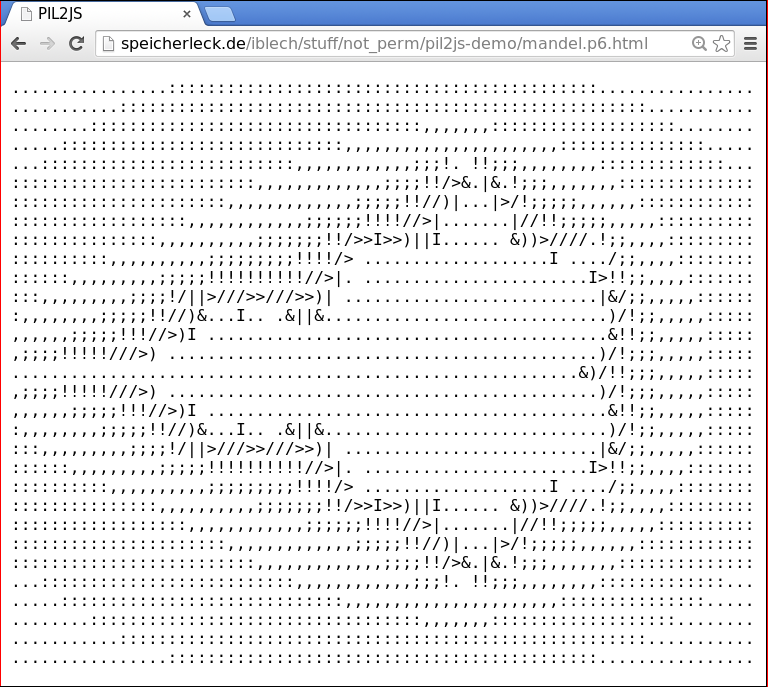
\includegraphics[scale=0.25]{images/mandel-in-the-browser}\end{center}

  \inputminted{perl}{code-snippets/day193-jsan.pl}
\end{frame}
% http://irclog.perlgeek.de/perl6/2005-07-17

\note{
  \begin{itemize}
    \justifying
    \scriptsize
    \item PIL2JS was written in Perl~5, in a style heavily influenced by
    Haskell. It used the Haskell part of Pugs to parse (and run BEGIN blocks)
    of Perl 6 code and translated the resulting PIL code (Pugs Intermediate
    Language) to JavaScript. Together with a runtime library in JavaScript,
    this allowed Perl~6 code to be run in the browser.
    \item Having the advantage of a later start, with more details of Perl~6's
    container binding semantics understood, it was the first backend to pass
    those tests. (See
    \url{https://github.com/perl6/roast/blob/master/S03-binding/arrays.t} for
    some of the binding features of Perl~6.)
    \item The first version was hacked together on a weekend and passed
    most of the basic ``sanity tests'', two days after putter (Mitchell N.
    Charity) started working on a PIL interpreter in Perl~5.
    \item Amazingly, a compiled version of the testsuite survived ten years of
    life: Run the tests yourself at
    \url{http://speicherleck.de/iblech/stuff/not_perm/pil2js-demo/}. \\ For the
    bulk of the tests, in the \texttt{t/} subdirectory, you have to add
    the entry \texttt{31.15.67.4 m19s28.vlinux.de} to your \texttt{/etc/hosts}.
  \end{itemize}
}

\note{
  \begin{itemize}
    \justifying
    \scriptsize
    \item JSAN was an attempt to bring a CPAN-like platform to JavaScript. The
    JavaScript backend was able to use JSAN modules.
    \item Foreshadowing node.js:
    \sourcedquote{It is entirely possible that the JavaScript backend may prove
    to be the most important one. [\ldots]
    Indeed, if JavaScript2 does survive the standardization
    process, it is entirely possible that it may become the next Ruby, because
    writing programs that run at both client and server side is a strong
    motivation -- the same reason to keep Pugs targetable to multiple
    backends.}{Audrey Tang}{October 30th,
    2005}{http://wayback.archive.org/web/20060924085336/http://use.perl.org/journal.pl?op=display&uid=1505&start=10}
  \end{itemize}
}

% XXX: Hackathons
% Vienna?
% Leo in June 2005
% Toronto in June 2005
% Liz in October 2005

\logo{}

\subsection{The end}

\begin{frame}[label=the-end]\frametitle{The end}
  \begin{Mdescription}{Beginning of 2007}
    \item[Beginning of 2007]
      Active development of Pugs stalls.
  \end{Mdescription}

  \begin{center}
    \emph{-- discussion only verbally --}
  \end{center}
\end{frame}

\note{
  \begin{itemize}
    \justifying
    \item For school reasons, I withdrew from Pugs development before its active phase
    ended. Therefore I'm not qualified to report on the reasons for its end
    and deem it unresponsible to speculate in public.
    \item Note that Pugs is still kept compatible with respect to new GHC
    releases.
  \end{itemize}
}

% Reasons may or may not include (sorted alphabetically):
%
% * "Low-hanging fruits" gradually vanished. Progress was not as rapid as
%   in the early days.
%
% * Audrey got ill.
%
% * Efforts were redirected to bringing some of Perl 6's unique features
%   to Perl 5.
%
% * Further development required advances in the host language, Haskell.
%
% * Missed insight: A Perl 6 compiler has to be tightly coupled with a
%   rules engine, to allow for the compile-time syntax modifications
%   which Perl 6 allows.
%
% Also see the thread http://perlmonks.org/?node_id=835731, containing posts
% from chromatic and Audrey. *Please* don't trust my assessment. I don't have
% any personal familiarity with the end of Pugs's active life and gathered
% those speculations only from various online sources.


\section{Pugs's unique culture}

\subsection{Test-driven development}

\begin{frame}\frametitle{Test-driven development}
  \begin{itemize}
    \item Tests as to do lists.
    \item Tests as bug reports.
    \item Tests as specification.
  \end{itemize}

  \begin{center}
    
\includegraphics[scale=0.5]{images/test-all-the-things.jpeg}
  \end{center}
\end{frame}

\note{
  \begin{itemize}
    \justifying
    \scriptsize
    \item One could upload test results to a public \emph{smoke server}.
    \item The neat visualization (using Test::TAP::HTMLMatrix, created
    specifically for Pugs) was interlinked with the design documents.
  \end{itemize}

  \vspace{-0.5em}
  \centering
  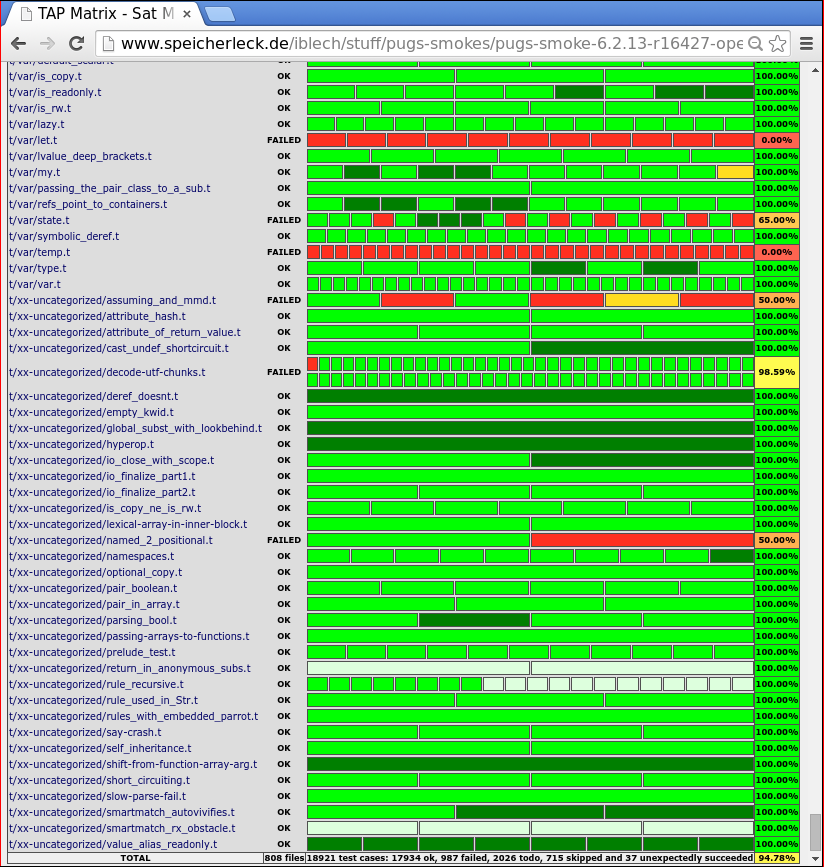
\includegraphics[scale=0.24]{images/test-matrix}
  \par
}

\subsection{Transparency}

{\setbeamertemplate{background canvas}{
\includegraphics[width=\paperwidth]{images/transparency}}
\begin{frame}\frametitle{Transparency}
  \begin{itemize}
    \item Audrey's journal (\href{http://pugs.blogs.com/}{\underline{link}}): \\
    \qquad\quad documenting progress, \\
    \qquad\quad\qquad\quad spreading excitement
    \item Public IRC logs
    \item svnbot, announcing new commits
    \item ``Private code $=$ dead code.'' ``url?''
  \end{itemize}
\end{frame}}


\subsection{Optimizing for fun}

\begin{frame}\frametitle{Pugs's unique culture}
  \begin{center}
    \Huge
    \only<1>{\hcancel{\scalebox{2.5}{-O\hil{2}}}{0pt}{3pt}{0pt}{-2pt}}
    \only<2>{\hcancel{\scalebox{2.5}{-O\hil{s}}}{0pt}{3pt}{0pt}{-2pt}}
  \end{center}
\end{frame}

\definecolor{mypurple}{RGB}{150,0,255}
{\setbeamercolor{frametitle}{bg=mypurple,fg=white}
\setbeamertemplate{background canvas}{
\includegraphics[width=\paperwidth]{images/mario.jpeg}}
\begin{frame}\frametitle{Optimizing for fun}
  \begin{center}
    \Huge
    \scalebox{2.5}{-O\hil{fun}!}
  \end{center}

  \begin{itemize}
    \item Liberal granting of commit bits.
    \item Forgiveness $>$ permission.
    \item ``Imagineering'', sketching ideas with code.
    \item Many subprojects, avoiding deadlocks.
  \end{itemize}

  \pause
  \centeredpar{0.85}{
    \hil{Audrey single-handedly bootstrapped a diverse and tight-knit
    community of lambdacamels, sharing a common vision and thoroughly
    enjoying their time.}
    Thank you, Audrey. $\heartsuit$
  }
\end{frame}}

\note{
  \begin{itemize}
    \justifying
    \item ``Patches are boring, commits are fun.''
    \item The diverse community was very welcoming. Trolls were hugged and
    turned into committers.
    \item Somebody would come to \#perl6 and mention that \$FEATURE
    does not work yet. Audrey would send them a commit bit, ask to create a
    test exemplifying the missing feature, and often implement the feature till
    the next day (or hour (or quarter of an hour)).
    \item People worked on the Haskell parts of the interpreter and the
    compiler, on unit tests, on porting and creating modules, on examples and
    documentation, on various backends (Perl~5 and JavaScript) written in
    Perl~5, on fun side projects (such as understanding type inference
    algorithms), and many other things.
    \item
    \href{https://speakerdeck.com/audreyt/ofun-optimizing-for-fun}{Audrey's
    slides \emph{-Ofun: Optimizing for Fun}} and Geoff Broadwell's
    \href{https://web.archive.org/web/20051125071047/http://www.oreillynet.com/pub/wlg/7996}{article
    on O'Reilly Network} are highly recommended reading.
  \end{itemize}
}

\note{
  \begin{center}
    
\includegraphics[scale=0.6]{images/trolling-perl6.jpeg}
  \end{center}
}

\note{
  \begin{itemize}
    \justifying
    \item \sourcedquote{One of my goals of this project is to keep it dual-cultured. So the
    source tree is managed with both svk and darcs; the build system requires
    both Perl5 and GHC; I will submit my Apocrypha series of design documents
    as monthly articles to both Perl.com and The Monad Reader; the project info
    is on both CPAN and the Haskell Wiki; etc, etc.}{Audrey Tang}{February 6st,
    2005}{http://wayback.archive.org/web/20050206202119/http://use.perl.org/~autrijus/journal/}

    \item \sourcedquote{In other news, Pugs was mentioned on The Haskell
    Sequence today. Indeed, I have noted that a significant part of questions
    asked in \#haskell are from camelfolks. Conversely, we saw a large influx
    from lambdafolks to \#perl6 as well. Lots of knowledge transfer is
    happening, which makes me really happy.}{Audrey Tang}{February 24th,
    2005}{http://pugs.blogs.com/pugs/2005/02/day_24_an_amazi.html}
  \end{itemize}
}

\note{
  \begin{itemize}
    \justifying
    \item Post on Lambda the Ultimate, a programming languages weblog:

    \sourcedquote{I'm a great fan of theoretical concepts like arrows,
    but at the same time I'm a self-employed programmer interested in solving
    my clients' problems.
    
    Pugs is notable in that it profitably uses recent developments such as
    GADTs and Template Haskell for an implementation of Perl6.
    
    I recently became a regular on the \#perl6 irc channel and soon after joined
    the list of committers.
    
    In just a few days I've seen a lot. I've seen enthusiastic members of the
    Perl community learning Haskell. I've seen myself learning Perl. I've also
    seen how daily Perl programmers work with abstractions like monad
    transformers. I've seen how some structures are easy to extend for
    programmers new to both the Pugs codebase and Haskell.}{Shae Errison (shapr)}{April 5st,
    2005}{http://lambda-the-ultimate.org/node/620}
  \end{itemize}
}

\note{
  \#haskell on 2013-03-23, \href{http://ircbrowse.net/browse/haskell?events_page=439213}{\underline{link}}:
  \begin{tabbing}
    \hil{$\langle$edwardk$\rangle$} \= \kill
    \hil{$\langle$edwardk$\rangle$} \> I found Haskell first through the existence of pugs. \\
    \hil{$\langle$elliott$\rangle$} \> perl, well known for attracting category theorists \\
    \hil{$\langle$edwardk$\rangle$} \> well, i was mining category theory at the time too. \\
    \hil{$\langle$shachaf$\rangle$} \> Pugs, well known for getting people into Haskell.
  \end{tabbing}

  \justifying
  Edward Kmett is well-known in the Haskell community. One of his hobbies is
  infusing Haskell's equivalent of CPAN with generalized abstract nonsense
  packages inspired by category theory, which somehow end up as dependencies
  for such mundane things as web frameworks.
  \par
}

\note{
  \begin{itemize}
    \scriptsize
    \justifying
    \item Other fun aspects of Pugs's culture: academic paper reading, game
    development, code obfuscation, Lord of the Rings poetry, other poetry
    (\href{https://github.com/audreyt/pugs/blob/master/docs/talks/larry_mariner.txt}{\uline{Larry
    was a mariner}}), videos
    (\href{https://github.com/iblech/talk-pugs-retrospective/raw/master/oscon05-stevan.mp4}{\uline{Fear
    and Loathing in Pugsland}}), hackathons (among others, with Elizabeth
    Mattijsen -- now, of course, a prolific Rakudo contributor), \ldots
  \end{itemize}

  \vspace{-1em}
  \inputminted{haskell}{code-snippets/day001-main.hs}
}


\section{Lasting contributions of Pugs}

\begin{frame}\frametitle{Lasting contributions of Pugs}
  \begin{itemize}
    \item Renewed interest in Perl 6.
    \item Major refinements of the specification.
    \pause
    \item \hil{The test suite.} Approximately 20\,000 unit tests.
    \pause
    \item The culture.
    \item Publicity for Haskell.
    \pause
    \item \hil{Moose.}

    \begin{center}
\includegraphics[scale=0.3]{images/moose.jpeg}\end{center}
  \end{itemize}
\end{frame}

\note{
  \begin{tabbing}
    \hil{$\langle$stevan$\rangle$} \= \kill
    \#perl6 on 2005-07-20: \\
    \hil{$\langle$stevan$\rangle$} \>
    geoffb: I think ``moose'' is a private joke between nothingmuch \\
    \> and himself :) \\\\
    \#perl6 on 2006-03-06: \\
    \hil{$\langle$stevan$\rangle$} \>
    audreyt: I have to run (dinnertime), but I have to show you \\
    \> Moose.pm soon, it is my (Class::MOP based) answer to Spiffy :)
  \end{tabbing}

  \justifying
  stevan is Stevan Little, nothingmuch is Yuval Kogman. Moose originated in
  Stevan's work on the Perl 6 metamodel (which governs objects, classes, and
  metaclasses).
  \par
}

\note{
  \justifying\scriptsize
  \sourcedquote{It came out of the Pugs project, which is a project that in
  about 2005 started. It was Audrey Tang who had decided that she wanted to
  implement Perl~6 in Haskell. So it was sort of a very fun project. Audrey
  coined the term “O-fun”, optimized for fun.\medskip

  And a lot of the goal of the project was to get some juice flowing back into
  the Perl 6 community and really get a working or a semi-working
  implementation so people could play with it.\medskip

  One of the things that I did in that project was to prototype the object
  system for Perl~6. I read over the Apocalypse~12, read up on a number of
  different object systems in different languages such as Smalltalk, CLOS,
  which is the Common Lisp Object System. Objective~C's object runtime,
  Ruby, Python, all those things. We were doing a lot of research at time and
  we tried to put a lot of that stuff, a lot of the good ideas, into the Perl~6
  object system.\medskip

  And then basically as the Pugs project started to peter out, I found myself
  going back to my work code, which was your basic vanilla Perl~5 OO. And I
  really craved all the features that I had been prototyping.\medskip

  So months here and months there, I fiddled around and I finally came up with
  a module called Class::MOP which is basically the basis on which Moose sits.
  And so a couple months after Class::MOP, we released Moose and sort of got
  running from there.}{Stevan Little}{December
  2010}{http://perlcast.com/2010/07/12/stevan-little-on-moose/}
  % This excerpt starts at offset 3:50.
}

\appendix

\begin{frame}[plain,noframenumbering]
  \begin{center}
    
\includegraphics[scale=0.5]{images/lambdacamel-small}
  \end{center}
\end{frame}

\note{
  This \emph{lambdacamel} illustration is by Carina Willbold. Feel free to use
  it in your talks! (CC BY)
}

\end{document}

http://www.slideshare.net/autang/pugs-a-perl-6-implementation
http://www.slideshare.net/autang/ofun-optimizing-for-fun
http://perlmonks.org/?node_id=835731

https://gist.github.com/quchen/5280339
trolling #haskell

http://developers.slashdot.org/story/05/10/09/1831219/optimizing-development-for-fun
frivolous toy interpreter

http://www.nntp.perl.org/group/perl.perl6.language/2005/02/msg19263.html
kudos to autrijus

pioneering techniques:
GADTs

fun:
slides "Perl 6, genau jetzt!"

porting modules
testing stuff
force_todo
some builtins
IRC library and bots
hyper operators
state/FIRST
macros
smokeserver
PIL2JS

http://pugs.blogs.com/pugs/2005/05/day_109_corouti.html
<iblech> Yeah, I start to grok Haskell :)
<autrijus> iblech++ # demonstrating that the productivity is really not me, it's really Haskell :)

http://perlmonks.org/?node=perl+oddities

http://strangelyconsistent.org/blog/happy-10th-anniversary-perl-6
https://www.fsf.org/blogs/community/recognizing-an-inspiring-woman-for-ada-lovelace-day-audrey-tang

chromatic in http://www.perl.com/pub/a/2005/07/28/test_builder_p6.html?page=3:
My productivity increased when Autrijus told me about Haskell's trace function.
He called it a refreshing desert in the oasis of referential transparency.
